\documentclass[final]{cvpr}

\usepackage{times}
\usepackage{epsfig}
\usepackage{graphicx}
\usepackage{amsmath}
\usepackage{amssymb}

% Include other packages here, before hyperref.

% If you comment hyperref and then uncomment it, you should delete
% egpaper.aux before re-running latex.  (Or just hit 'q' on the first latex
% run, let it finish, and you should be clear).
\usepackage[pagebackref=true,breaklinks=true,colorlinks,bookmarks=false]{hyperref}

%%%%%%%%% PAPER ID  - PLEASE UPDATE
% \def\cvprPaperID{****} % *** Enter the CVPR Paper ID here
%\def\httilde{\mbox{\tt\raisebox{-.5ex}{\symbol{126}}}}

\def\cvprPaperID{****} % *** Enter the CVPR Paper ID here
\def\confYear{CVPR 2024}

\begin{document}

%%%%%%%%% TITLE - PLEASE UPDATE
\title{Real and Fake Face Detection}  % **** Enter the paper title here

\author{Person1\\
1234567\\
Master in Data and Computer Science\\
{\tt\small Person1@i1.org}
\and
Person1\\
1234567\\
Master in Data and Computer Science\\
{\tt\small Person1@i2.org}
\and
Person1\\
1234567\\
Master in Data and Computer Science\\
{\tt\small Person1@i2.org}
\and
Person1\\
1234567\\
Master in Data and Computer Science\\
{\tt\small Person1@i2.org}
\and
Mentor: Person 5
}


\maketitle
\thispagestyle{empty}


%%%%%%%%% BODY TEXT - ENTER YOUR RESPONSE BELOW
\section{Abstract}

\section{Introduction}

After receiving paper reviews, authors may optionally submit a rebuttal to address the reviewers' comments, which will be limited to a {\bf one page} PDF file.  Please follow the steps and style guidelines outlined below for submitting your author response.

Note that the author rebuttal is optional and, following similar guidelines to previous CVPR conferences, it is meant to provide you with an opportunity to rebut factual errors or to supply additional information requested by the reviewers. It is NOT intended to add new contributions (theorems, algorithms, experiments) that were not included in the original submission. You may optionally add a figure, graph or proof to your rebuttal to better illustrate your answer to the reviewers' comments.

Per a passed 2018 PAMI-TC motion, reviewers should not request additional experiments for the rebuttal, or penalize authors for lack of additional experiments. This includes any experiments that involve running code, e.g., to create tables or figures with new results.  \textbf{Authors should not include new experimental results in the rebuttal}, and reviewers should discount any such results when making their final recommendation. Authors may include figures with illustrations or comparison tables of results reported in the submission/supplemental material or in other papers. 

The rebuttal must adhere to the same blind-submission as the original submission and must comply with this rebuttal-formatted template.

%-------------------------------------------------------------------------

\subsection{Sample}
Sample

%------------------------------------------------------------------------
\section{Related Work}

\section{Method}
\subsection{Datasets}
\cite[Dataset]{kaggledatasetRealAndFakeFaceDetection}

\subsubsection{Simple CNN}

A simple CNN network can be used to test the correctness of program exectution and observe the flow of data. Because of its brief structure, it can significantly reduce the cost of computing resources. At the same time, it can alos be used as one of the benchmark performance indicators for comparison and analysis with other types of subsequent network models.

This convolutional neural network is designed for image classificaion, structured with an input layer which taks 3-channel RGB images, followed by three convolutional layers, each with a 3x3 kernal and padding of 1, progressively increasing the number of filters from 32 to 64 and finally 128. Each convolutional layer is followed by a ReLU activation function and a 2x2 max pooling layer. The output is flattened and passed throught two fully connected layers. The first FC layer transforms the feature map into 512 features, followed by another ReLU, and the second FC layer reduces it to 2 outputs for classification. 

\subsubsection{Improved CNN}

The Improved CNN represents an enhancement of the previous 'SimpleCNN' model. it is designed to achieve better performance by adopting serveral architectural adjustments to increase the network's capacity and reduce overfitting.

Compared with the basic version of CNN, the improved version of convolutional neural network has been improved in the following aspects: An additional convolutional layer has been introduced; The depth is increased with 256 filters; Each convolutional layer is now followed by a batch normalization layer; A dropout layer with a rate is introduced before the first fully connected layer; Also an increased fully connected layer capacity, transforms the feature maps into a larger dimensional space.


\section{Experiments}

\subsection{Dataset 1}

WIP

\begin{figure}[t]
   \centering
   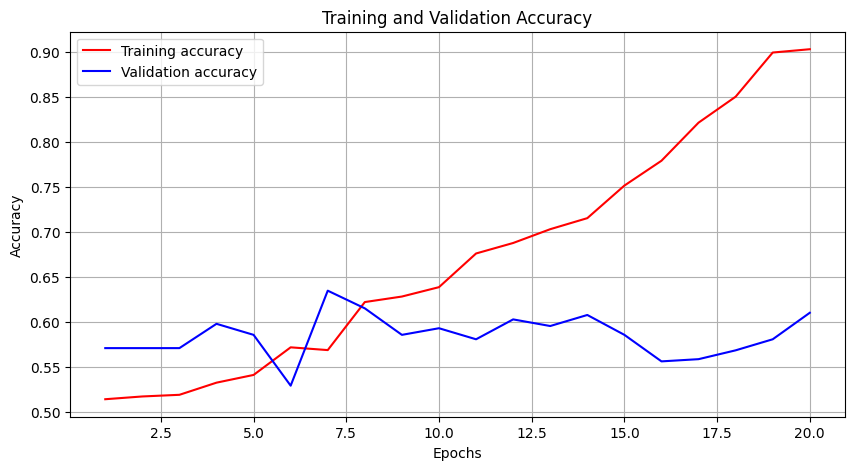
\includegraphics[width=0.9\linewidth]{img/ex-d1-simplecnn-accuracy-results.png}
   \caption{Training and Validation results of simple CNN with the compact dataset}
   \label{fig:ex-d1-simplecnn-results}
\end{figure}

\begin{figure}[t]
   \centering
   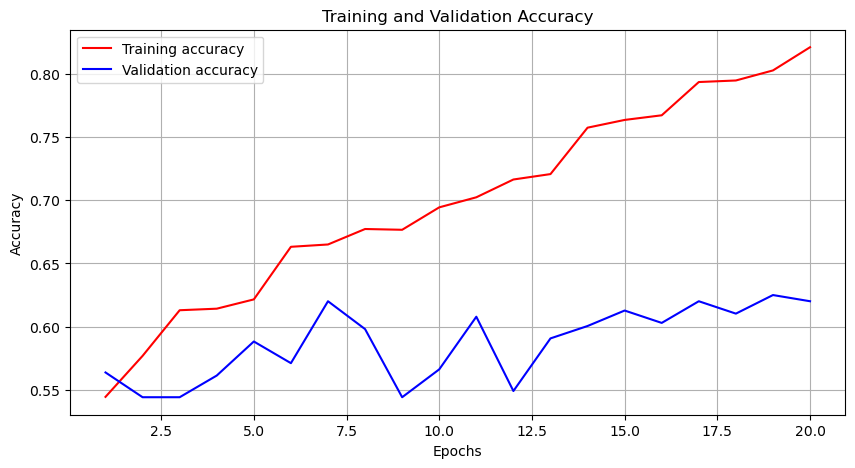
\includegraphics[width=0.9\linewidth]{img/ex-d1-improvedcnn-accuracy-results.png}
   \caption{Training and Validation results of improved CNN with the compact dataset}
   \label{fig:ex-d1-improvedcnn-results}
\end{figure}

% \begin{figure}[t]
%    \centering
%    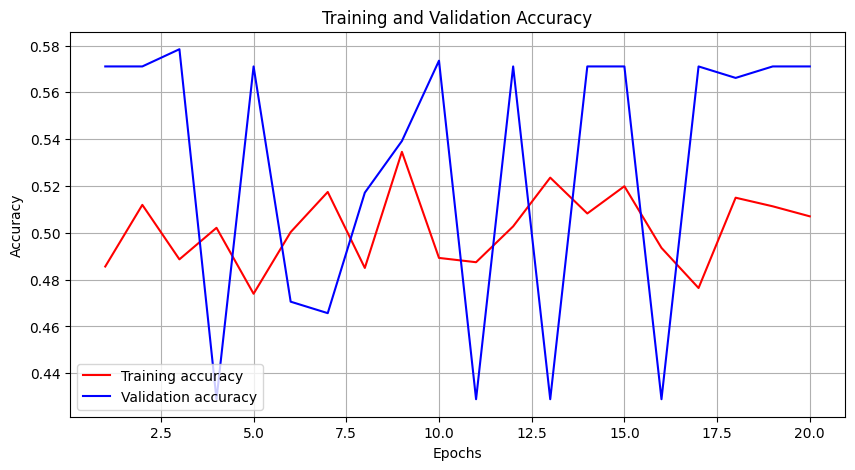
\includegraphics[width=0.9\linewidth]{img/ex-d1-gramnet51-accuracy-results.png}
%    \caption{Training and Validation results of GramNet51 with the compact dataset}
%    \label{fig:ex-d1-gramnet51-results}
% \end{figure}

% \begin{figure}[t]
%    \centering
%    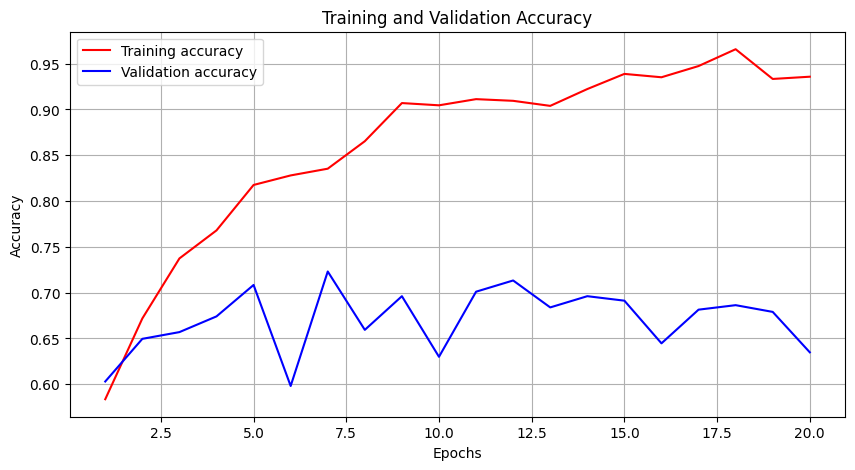
\includegraphics[width=0.9\linewidth]{img/ex-d1-MobileNetV2-accuracy-results.png}
%    \caption{Training and Validation results of MobileNetV2 with the compact dataset}
%    \label{fig:ex-d1-MobileNetV2-results}
% \end{figure}

\subsection{Dataset 2}

WIP

\begin{figure}[t]
   \centering
   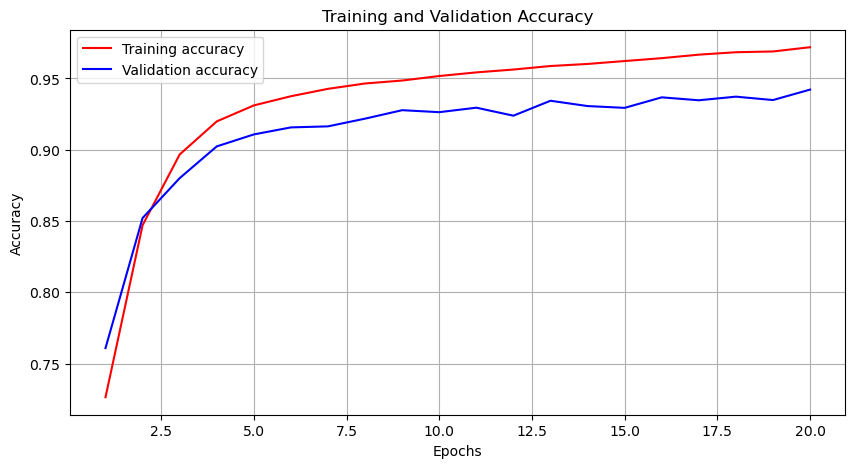
\includegraphics[width=0.9\linewidth]{img/ex-d2-simplecnn-accuracy-results.png}
   \caption{Training and Validation results of simple CNN with the large-scale dataset}
   \label{fig:ex-d2-simplecnn-results}
\end{figure}

\begin{figure}[t]
   \centering
   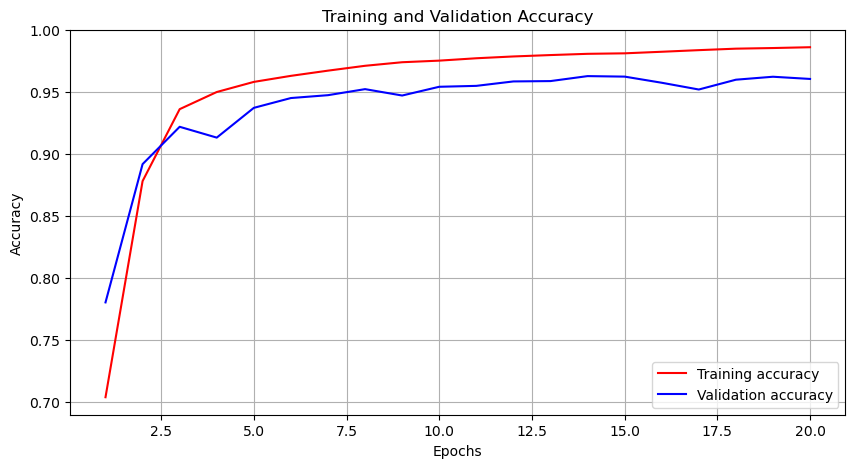
\includegraphics[width=0.9\linewidth]{img/ex-d2-improvedcnn-accuracy-results.png}
   \caption{Training and Validation results of improved CNN with the large-scale dataset}
   \label{fig:ex-d2-improvedcnn-results}
\end{figure}

% \begin{figure}[t]
%    \centering
%    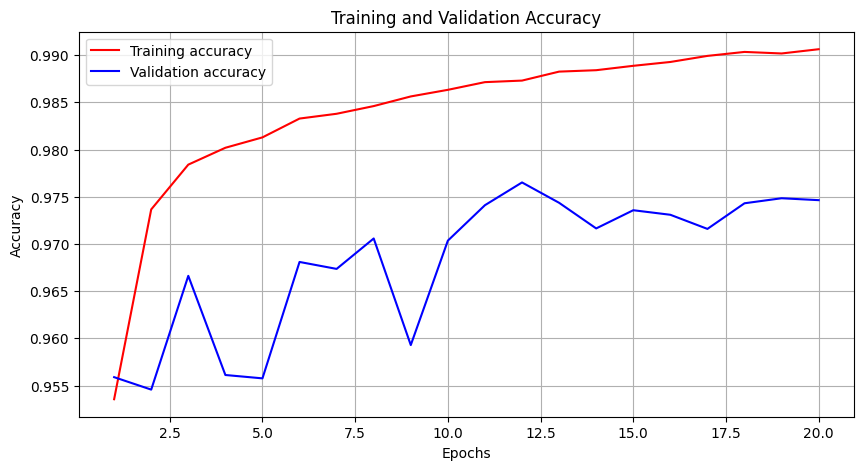
\includegraphics[width=0.9\linewidth]{img/ex-d2-mobilenetv2-accuracy-results.png}
%    \caption{Training and Validation results of MobileNetV2 with the large-scale dataset}
%    \label{fig:ex-d2-MobileNetV2-results}
% \end{figure}


\subsection{Cross-datasets Training}



\subsection{Dataset generated by GAN network}

\section{Findings}

{\bf Make sure to update the paper title and paper ID in the appropriate place in the tex file.}

All text must be in a two-column format. The total allowable width of the text
area is $6\frac78$ inches (17.5 cm) wide by $8\frac78$ inches (22.54 cm) high.
Columns are to be $3\frac14$ inches (8.25 cm) wide, with a $\frac{5}{16}$ inch
(0.8 cm) space between them. The top margin should begin
1.0 inch (2.54 cm) from the top edge of the page.  The bottom margin should be
1-1/8 inches (2.86 cm) from the bottom edge of the page for $8.5 \times
11$-inch paper; for A4 paper, approximately 1-5/8 inches (4.13 cm) from the
bottom edge of the page.

Please number all of your sections and any displayed equations.  It is important
for readers to be able to refer to any particular equation.

Wherever Times is specified, Times Roman may also be used.  Main text should be
in 10-point Times, single-spaced. Section headings should be in 10 or 12 point
Times.  All paragraphs should be indented 1 pica (approx. 1/6 inch or 0.422
cm).  Figure and table captions should be 9-point Roman type as in
Figure~\ref{fig:onecol}.


List and number all bibliographical references in 9-point Times, single-spaced,
at the end of your response. When referenced in the text, enclose the citation
number in square brackets, for example~\cite{Authors14}.  Where appropriate,
include the name(s) of editors of referenced books.

\begin{figure}[t]
\begin{center}
\fbox{\rule{0pt}{1in} \rule{0.9\linewidth}{0pt}}
   %\includegraphics[width=0.8\linewidth]{egfigure.eps}
\end{center}
   \caption{Example of caption.  It is set in Roman so that mathematics
   (always set in Roman: $B \sin A = A \sin B$) may be included without an
   ugly clash.}
\label{fig:long}
\label{fig:onecol}
\end{figure}


%-------------------------------------------------------------------------
\subsection{Illustrations, graphs, and photographs}

All graphics should be centered.  Please ensure that any point you wish to make is resolvable in a printed copy of the response.  Resize fonts in figures to match the font in the body text, and choose line widths which render effectively in print.  Many readers (and reviewers), even of an electronic copy, will choose to print your response in order to read it.  You cannot insist that they do otherwise, and therefore must not assume that they can zoom in to see tiny details on a graphic.

When placing figures in \LaTeX, it's almost always best to use \verb+\includegraphics+, and to specify the  figure width as a multiple of the line width as in the example below



{\small\begin{verbatim}
   \usepackage[dvips]{graphicx} ...
   \includegraphics[width=0.8\linewidth]
                   {myfile.eps}
\end{verbatim}
}

\section{Conclution}

{\small
\bibliographystyle{ieee_fullname}
\bibliography{egbib}
}




\end{document}
